\section*{Kommunikation}
\begin{frame}{Kommunikation}{Anforderungen}
  \begin{itemize}
    \item Controller -> PC
    \begin{itemize}
    \item Sensordaten
    \item Wiederholt
    \item Erweiterbarkeit
    \end{itemize}
    \item PC -> Controller
    \begin{itemize}
      \item Regelungsparameter
      \item Sporadisch
    \end{itemize}
  \end{itemize}
\end{frame}
\begin{frame}{Kommunikation}{Entwurf}
  \begin{itemize}
    \item Physical Layer
    \begin{itemize}
      \item UART-Baustein des $\mu$-Controllers via USB
      \item DAVE APP zur Parametrierung
    \end{itemize}
    \item Data Link Layer
    \begin{itemize}
      \item Eigens definiertes Frame-Format
    \end{itemize}
  \end{itemize}
  \begin{center}
    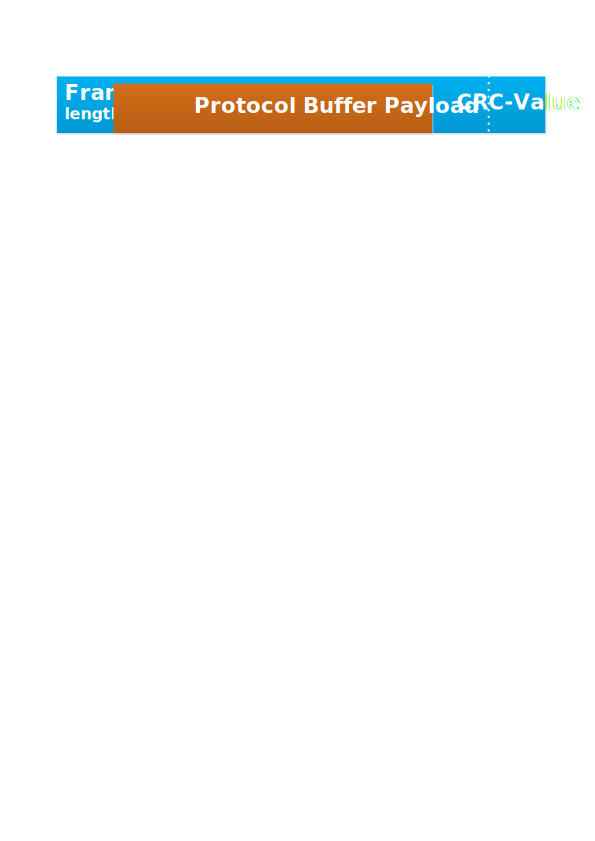
\includegraphics[width=\textwidth]{../communication/MessageFormat}
  \end{center}
\end{frame}
\begin{frame}{Kommunikation}{Entwurf}
  \begin{itemize}
    \item Restliche Layer
    \begin{itemize}
    \item Keine Adressierung, da genau zwei Teilnehmer
    \item Keine Sessions
    \item Keine Flusskontrolle
    \end{itemize}
    \item Payload: Protocol Buffer Nachricht
    \begin{itemize}
      \item Flexibilität und Erweiterbarkeit
      \item Performance
    \end{itemize}
  \end{itemize}
\end{frame}
\begin{frame}[fragile]{Kommunikation}{Entwurf}
  \begin{columns}[T]
  \begin{column}{5cm}
    \begin{itemize}
      \item Sensordaten
    \end{itemize}
    \begin{lstlisting}
    //defining an entry of the data table
    message DataEntry{
	    uint32 SensorId = 1;
	    double Data = 2;
    }
    //defining the real message
    message SensorMsg{
	    //Upcounting Nr
	    uint64 SequenceNr = 1;
	    //all Data
	    repeated DataEntry DataTable = 2;
    }
    \end{lstlisting}
  \end{column}
  \begin{column}{5cm}
    \begin{itemize}
      \item Parameter
    \end{itemize}
    \begin{lstlisting}
    //defining the parameter message
    message RegParams{
	    uint32 target = 1;
	    float paraP = 2;
	    float paraI = 3;
	    float paraD = 4;
	    float tgtVal = 5;
    }
    \end{lstlisting}
  \end{column}
  \end{columns}
\end{frame}
\begin{frame}{Kommunikation}{Implementierung}
  \begin{itemize}
    \item Frameaufbau f\"ur Sensordaten erweitert
  \end{itemize}
  \centering{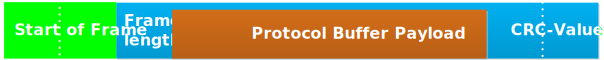
\includegraphics[width=\textwidth]{../communication/MessageFormat_enhanced}}
  \begin{itemize}
    \item PC: C\#-Bibliothek
    \begin{itemize}
    \item SerialPort-Objekt
    \end{itemize}
    \item Controller: C-Funktionen
    \begin{itemize}
      \item DAVE APP f\"ur UART
      \item DAVE APP f\"ur CRC
    \end{itemize}
  \end{itemize}
\end{frame}
